\subsection{How is the concept of monitoring implemented in Ambari and Chukwa?}
\label{subsec:Implementation}

\subsubsection{Ambari}
\amb is an open source framework that allows the User to monitore, manage and install Hadoop.[1] It has the ability to start, stop and configurate Hadoop processes automatically on clusters, without any intervention of the user.\amb was founded to simplify the use of Hadoop.[12]
\\
\amb architecture can be divided in connected parts. First the \amb Web which is the main platform for Users to log in and give up request that should be run through \amb.[12] Secondly the \amb Server, which is divided into smaller parts itself. The API or REST API is connected to different Web applications, the most important one of this is \amb Web. Other interfaces like Microsoft System Center, are applications that allows the user to analyse the data furthermore the capability of Hadoop.[1] The results of the analyse is accessible through \amb Web, on the monitroing screens.[12]
\\
The connection between \amb and Hadoop is done by the \amb Agents. \amb Server installs on each hast an \amb Agent, that gives every few seconds a heartbeat to the server; the server answers with an instruction for the Agent or it sends a confirmation about his current life-status. All hostes are connected to the Clusters by Hadoop.
\\
\begin{figure}[hbt]
  \centering
  % https://docs.google.com/open?id=1A3TbXPEQeknqWxxX811XHG7pcQOuMEFDmo_hl8LlfYk
  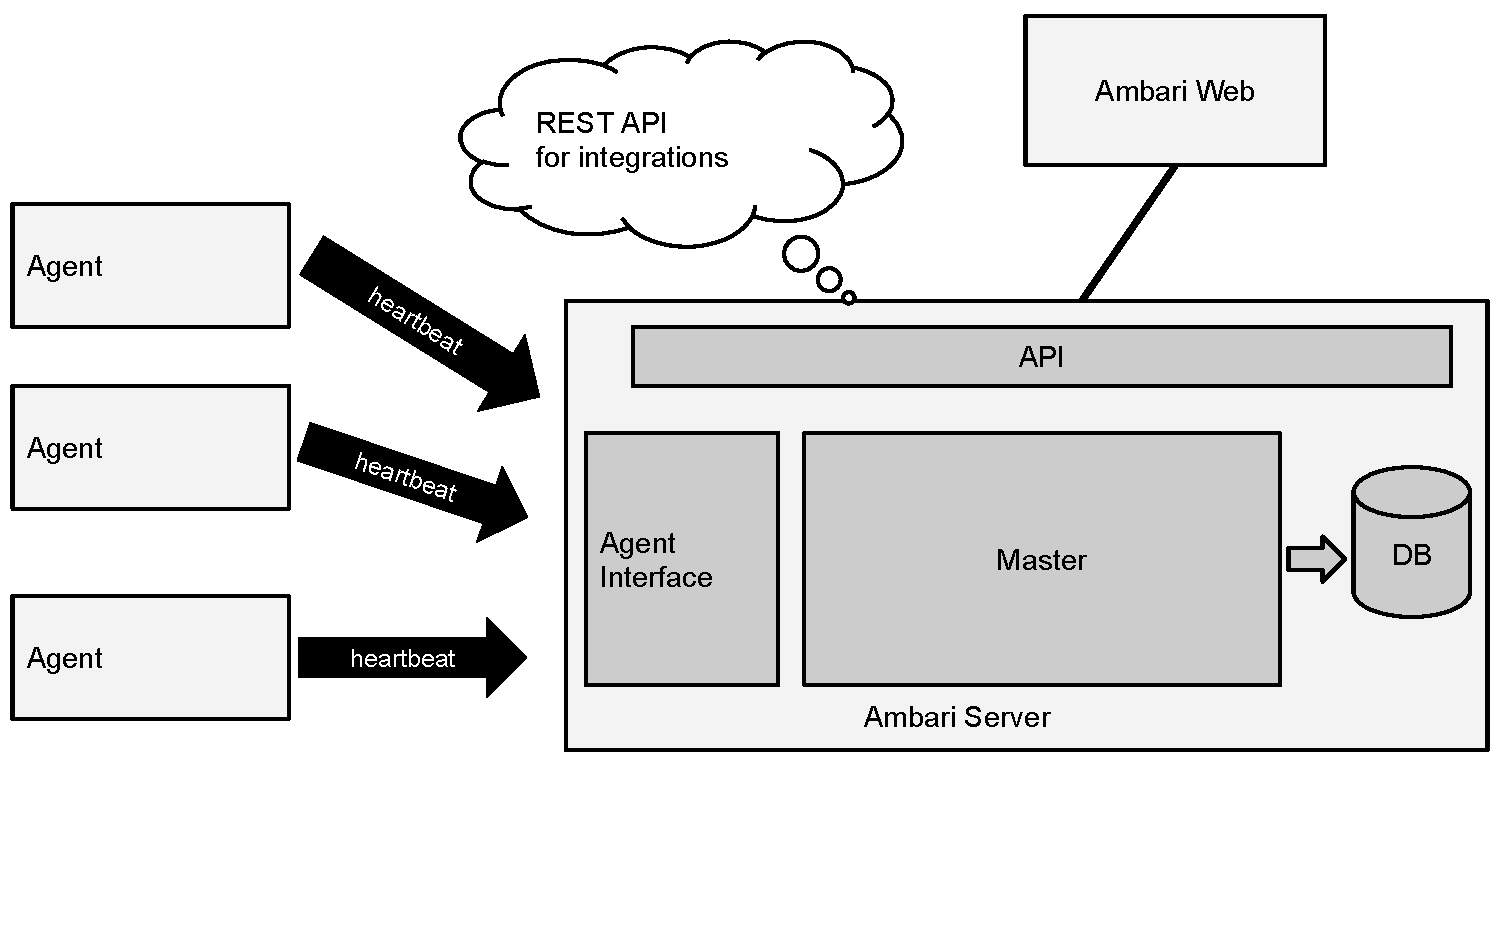
\includegraphics[width=\linewidth,clip=true,trim=0 3cm 0 0]{images/AmbariArchitecture}
  \caption{Ambaris Architecture~\cite{Sako}}
  \label{fig:AmbariArchitecture}
\end{figure}

The concept of monitoring is given in two specific ways with \amb\. \amb has the knowledge about any cluster health and its data. It can provide and improve the health situation of a Hadoop cluster and analyse the data in ways there are useful for the user. The user has an overview on the current situation through the Web application. \amb divides to monitoring Prozess in three parts. The first one is the List of all the Application \amb is running on any of the connected Clusters. It shows the name, status und number of clusters that are in default, and need to get be fixed. The second part is explain all the technical details about the application, such as storing space and running time. The last part is aimed to show illustratively how long and effective an application has been running on any clusters. Based on this data the user can give up requests to change the applications or add more clusters into one process, through the API. \amb then will install automatically an new application to the cluster on sending heartbeat information to the \amb Agent. 

\subsubsection{Chukwa}
\chuklong is ``a data collection system for monitoring and analyzing large distributed systems.''~\cite{Boulona}
It is built to support log handling on scalable Hadoop clusters. \chuk is developed at Yahoo! and ``is built on top of HDFS and Map-Reduce.''~\cite{Rabkin2008a}
Its main non-functional goals are low footprint on System Usage (less than 5\%) and minimal changes to user workflow.~\cite{Rabkin2010}


\begin{figure}[hbt]
  \centering
  % https://docs.google.com/open?id=11xCUWZ94zbUa4eqhoScjMmfIL2pI-IkDx02qvcCXohY
  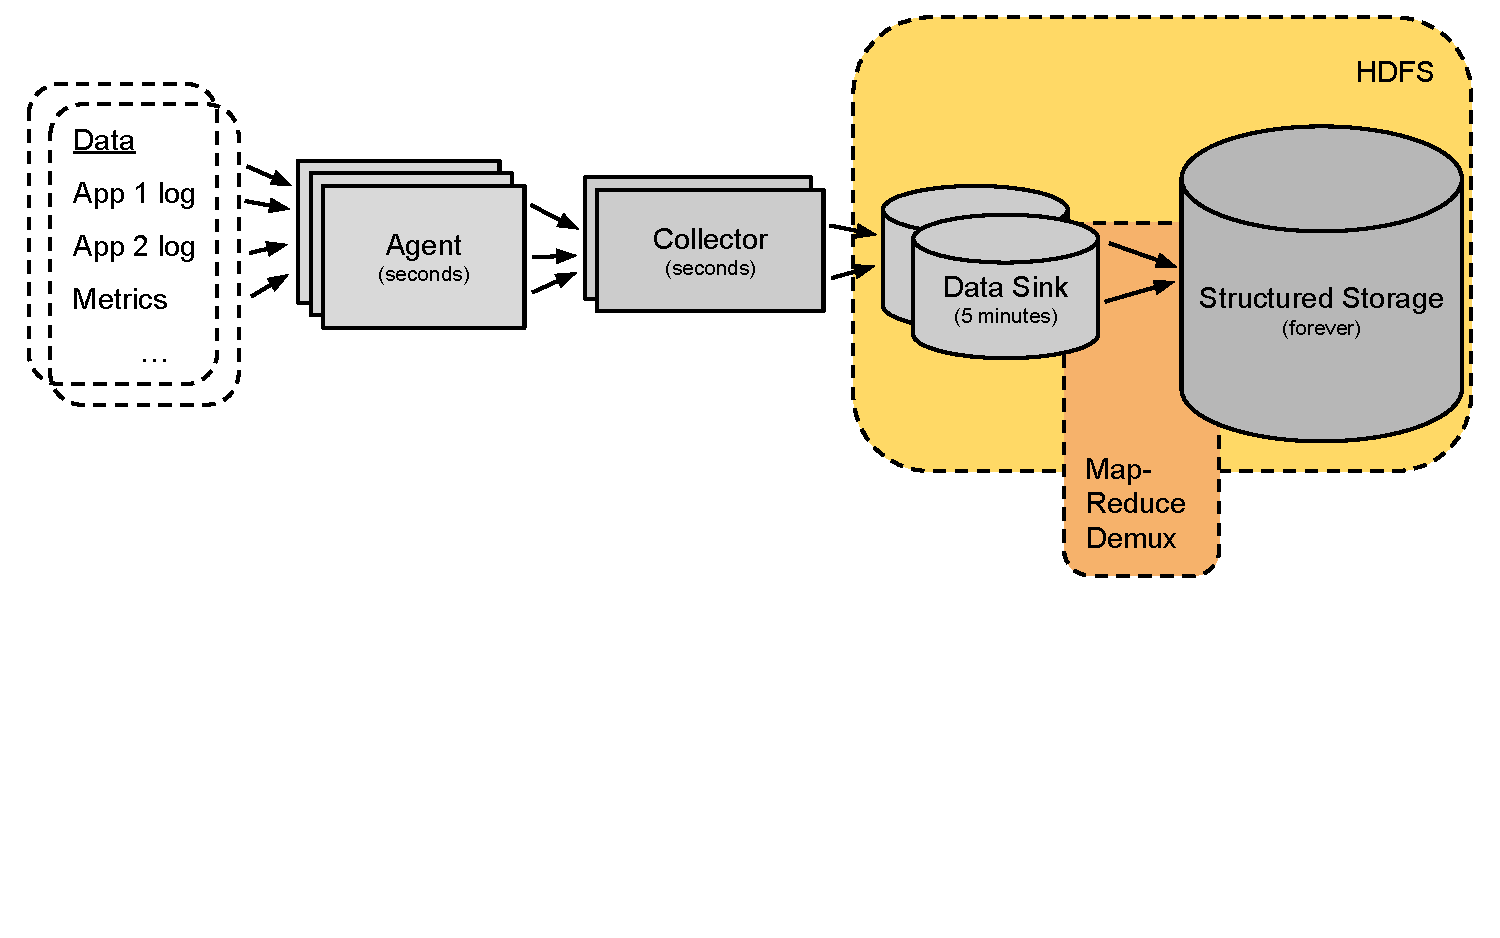
\includegraphics[width=\linewidth,clip=true,trim=0 6cm 0 0]{images/ChukwaArchitecture}
  \caption{Chukwas Architecture~\cite{Rabkin2008}}
  \label{fig:ChukwaArchitecture}
\end{figure}
